% --- LaTeX CV Template - S. Venkatraman ---

% --- Set document class and font size ---

\documentclass[letterpaper, 11pt]{article}

% --- Package imports ---

\usepackage[utf8]{inputenc}
\usepackage[T1]{fontenc}
\usepackage{hyperref, enumitem, longtable, amsmath, array}

% --- Page layout settings ---

% Set page margins
\usepackage[left=0.7in, right=0.8in, bottom=.8in, top=0.8in, headsep=0in, footskip=.2in]{geometry}
\usepackage{graphicx}
\usepackage{multirow}

% Set line spacing
\renewcommand{\baselinestretch}{1.2}

% --- Page formatting settings ---

% Set link colors
\usepackage[dvipsnames]{xcolor}
\hypersetup{colorlinks=true, linkcolor=MidnightBlue, urlcolor=MidnightBlue}

% Set font to Libertine, including math support
\usepackage{libertine}
\usepackage[libertine]{newtxmath}

% Remove page numbering
\pagenumbering{gobble}

% Define font size and color for section headings
\newcommand{\headingfont}{\Large\color{OliveGreen}}

% --- CV section settings ---

% Note: each section of this table (Education, Awards, Publications etc.) is 
% stored in a two-column table. The left-hand column is narrow (1 inch) and is 
% meant to store dates. The right-hand column is wide (5.2 inches) and stores 
% the main text.  Sections in which each entry might have multiple lines 
% (e.g., Education) are stored in a 'SectionTable' environment). Sections in 
% which each entry might just have one line are stored in a 'SectionTableSingleSpace'
% environment. The only difference between the two environments is the line 
% spacing between each entry. Both environments take one argument, which is the
% title of the section. See main document for how these environments are used.

% Define settings for left-hand column in which dates are printed
\newcolumntype{R}{>{\raggedleft}p{1in}}

% Define 'SectionTable' environment
\newenvironment{SectionTable}[1]{
	\renewcommand*{\arraystretch}{1.7}
	\setlength{\tabcolsep}{10pt}
	\begin{longtable}{Rp{5.2in}} & #1 \\}
{\end{longtable}\vspace{-1.5cm}}

% Define 'SectionTableSingleSpace' environment
\newenvironment{SectionTableSingleSpace}[1]{
	\renewcommand*{\arraystretch}{1}
	\setlength{\tabcolsep}{10pt}
	\begin{longtable}{Rp{5.2in}} & #1 \\[0.6em]}
{\end{longtable}\vspace{-3cm}}

% --- Document starts here ---

\begin{document}

% --- Name and contact information ---



\begin{SectionTable}{\Huge Michiel De Wilde} 
\end{SectionTable}\vspace{1.5cm}
\begin{tabular}{p{80pt}p{200pt}}
  \multirow{2}{*}{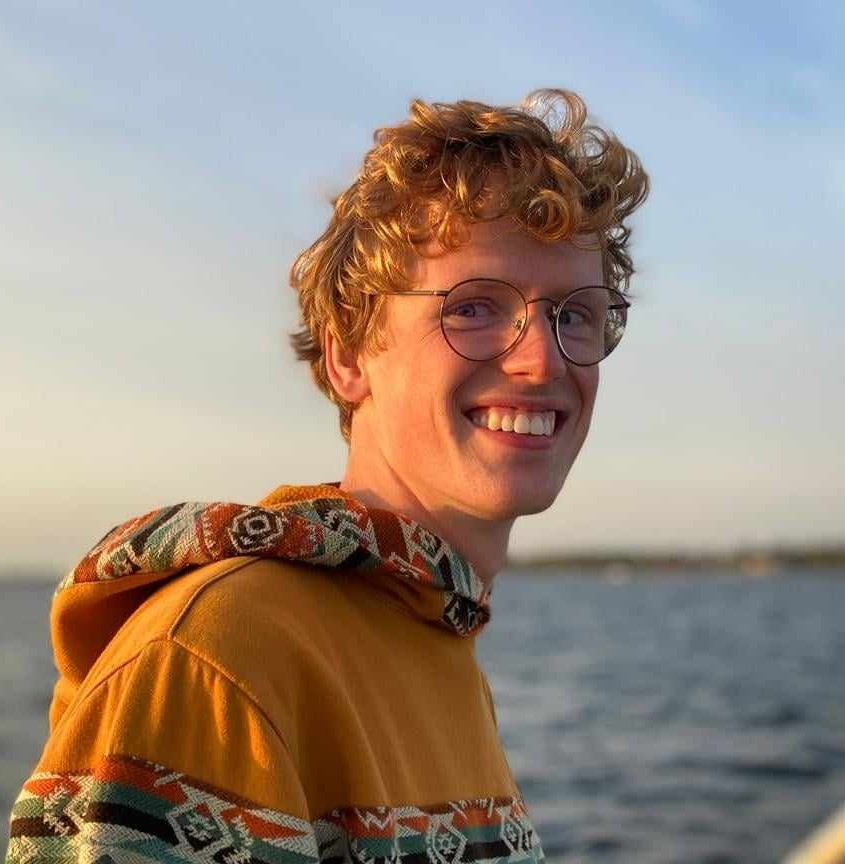
\includegraphics[width=80pt]{../assets/profile.jpg}} & \textbf{Contact Information} \\
  & \textbf{Email:} michiel.dewilde@ist.ac.at \\
  & \textbf{Phone:} +32 468 46 15 85 \\
  & \textbf{Citizenship:} Belgium
\end{tabular}
% --- Section: Research interests ---
\vspace{-0.8cm}
\begin{SectionTable}{\headingfont Research interests}
& Mathematical physics: Quantum many-body-systems, Topological phases

Side project: Astrophysics: stellar and solar flares. 
\end{SectionTable}

% --- Section: Education ---

\begin{SectionTable}{\headingfont Education}
2025 -- present & 
\textbf{ISTA} -- Kosterneuburg, Austria \newline
PhD with Robert Seiringer \newline 
% \textit{Project: Classification of Symmetry Protected Topological Phases in 2D}\newline
% Mentor: Professor Wojciech De Roeck.  
\\


2023 -- 2025 & 
\textbf{KU Leuven} -- Leuven, Belgium \newline
Master in Mathematics \textit{Summa cum Laude} \newline 
\textit{Project: Classification of Symmetry Protected Topological Phases in 2D}\newline
Mentor: Professor Wojciech De Roeck.  \\

2020 -- 2023 & 
\textbf{KU Leuven} -- Leuven, Belgium \newline
Bachelor in Physics, \textit{Magna cum laude}. \newline 
\textit{Project: Entanglement and topology
in quantum spin systems: Toric code.}\newline
Mentor: Dr. Bruno de Oliveira Carvalho.  \\

2020 -- 2023 & 
\textbf{KU Leuven} -- Leuven, Belgium \newline
Bachelor in Mathematics, \textit{Magna cum laude} \newline 
\textit{Project: Optically thick Radiative
Transfer in stars}\newline
Mentor: Professor Malcolm Druett.  \\


% --- Un-comment the next few lines if you want to include some courses you've taken ---

% & \textbf{Extra Credits}
    
%     \renewcommand{\arraystretch}{0.75}
% \begin{tabular}{llll}
% 2024-2025 & Mathematical Logic & 6 ECTS& - \\
% 2024-2025 & Avanced Quantum Field Theory & 6 ECTS &- \\
% 2024-2025 & Operator Algebras & 6 ECTS& - \\ 
% 2024-2025 & Condensed Matter Theory & 6 ECTS& - \\
% 2024-2025 & Algebraic Number Theory & 6 ECTS& - \\
% 2023-2024 & Riemann Surfaces & 6 ECTS &19/20 \\
% 2023-2024 & Relativity & 6 ECTS &17/20 \\
% 2023-2024 & Advanced Statistical Mechanics & 6 ECTS& 18/20 \\ 
% 2022-2023 & Algebra II& 6 ECTS & 16/20\\
% 2022-2023 & Particle Physics & 3 ECTS & 16/20\\
% 2022-2023 & Introduction to General Relativity & 3 ECTS & 16/20\\
% 2021-2022 & Number Theory & 6 ECTS & 20/20\\
% \end{tabular}


\end{SectionTable}

% --- Section: Awards, scholarships, etc ---

% \begin{SectionTableSingleSpace}{\headingfont Honors and scholarships}
% 2021 & 
% Award 1 (Organization that gave you the award)\newline
% \textit{Maybe this award needs a short description}. \\

% 2020 &
% Award 2 (Organization that gave you the award; \href{https://en.wikibooks.org/wiki/LaTeX/Hyperlinks}{link if you want}) \\

% 2019 &
% Award 3 (Organization that gave you the award) \\

% 2018 &
% Award 4 (Organization that gave you the award) \\

% 2017 &
% Award 5 (Organization that gave you the award)
% \end{SectionTableSingleSpace}

% --- Section: Publications ---

\newpage\begin{SectionTable}{\headingfont Publications}
% BEGIN GENERATED PUBLICATIONS
% This block is generated by scripts/build_cv.py. Edit assets/publications.js or
% scripts/cv-extra-publications.json, then run python scripts/build_cv.py.
2026 &
\textbf{Synthesizing Sun-as-a-star flare spectra from high-resolution solar observations (Corrigendum)} \newline
M. De Wilde, A. G. M. Pietrow, M. K. Druett, A. Pastor Yabar, J. Koza, I. Kontogiannis, O. Andriienko, A. Berlicki, A. R. Brunvoll, J. de la Cruz Rodríguez, J. Thoen Faber, R. Joshi, D. Kuridze, D. Nóbrega-Siverio, L. H. M. Rouppe van der Voort, J. Rybák, E. Scullion, A. M. Silva, Z. Vashalomidze, A. Vicente Arévalo, A. Wiśniewska, R. Yadav, T. V. Zaqarashvili, J. Zbinden, E. S. Øyre. \newline
\href{https://doi.org/10.1051/0004-6361/202660990e}{\textit{Astronomy \& Astrophysics}}. \\
2026 &
[under review] \textbf{On the effects of spherical geometry on coronal mass ejection detection} \newline
A. G. M. Pietrow, M. De Wilde, M. Druett, H. Eklund, J. D. Alvarado-Gomez, V. Fedun. \newline
\textit{Nature Astronomy}. \\
2026 &
\textbf{Classification of Locality Preserving Symmetries on Spin Chains} \newline
Alex Bols, Wojciech De Roeck, Michiel De Wilde, Bruno de O. Carvalho. \newline
\href{http://dx.doi.org/10.1007/s00220-025-05503-2}{\textit{Communications in Mathematical Physics}}. \\
2026 &
\textbf{Arbitrary harmonic functions as Bose–Einstein condensates} \newline
Michiel De Wilde, Robert Seiringer. \newline
\href{https://doi.org/10.1063/5.0325354}{\textit{Journal of Mathematical Physics}}. \\
2026 &
[preprint] \textbf{A complete classification of 2d symmetry protected states with symmetric entanglers} \newline
Alex Bols, Wojciech De Roeck, Michiel De Wilde, Bruno de O. Carvalho. \newline
\href{http://arxiv.org/abs/2603.09959v1}{\textit{arXiv}}. \\
2025 &
\textbf{Synthesizing Sun-as-a-star flare spectra from high-resolution solar observations} \newline
M. De Wilde, A. G. M. Pietrow, M. K. Druett, A. Pastor Yabar, J. Koza, I. Kontogiannis, O. Andriienko, A. Berlicki, A. R. Brunvoll, J. de la Cruz Rodríguez, J. Thoen Faber, R. Joshi, D. Kuridze, D. Nóbrega-Siverio, L. H. M. Rouppe van der Voort, J. Rybák, E. Scullion, A. M. Silva, Z. Vashalomidze, A. Vicente Arévalo, A. Wiśniewska, R. Yadav, T. V. Zaqarashvili, J. Zbinden, E. S. Øyre. \newline
\href{https://doi.org/10.1051/0004-6361/202554870}{\textit{Astronomy \& Astrophysics}}. \\
% END GENERATED PUBLICATIONS
\end{SectionTable}

%  --- Sectoin: Talks --------------
\begin{SectionTable}{\headingfont Talks}
% BEGIN GENERATED TALKS
% This block is generated by scripts/build_cv.py. Edit scripts/talks.json,
% then run python scripts/build_cv.py.
24/03/2026 &\textbf{Mathematical Physics \& Analysis Seminar (ISTA)}\newline
Title: Arbitrary harmonic functions as Bose-Einstein condensates\\

13/03/2026 &\textbf{Solar-stellar and star-planet connections: Mind the gap (Royal Astronomical Society)}\newline
Title: Synthesizing Sun-as-a-star flare spectra from high-resolution solar observations\\

15/10/2025 &\textbf{MIXed Colloquium (ISTA)}\newline
Title: Classification of locality-preserving symmetries on spin chains\\
% END GENERATED TALKS
\end{SectionTable}

% --- Section: Research experience ---

\begin{SectionTable}{\headingfont Internship}
2023 -- 2025 &
\textbf{Using spatially resolved solar flare data to assess spectral signatures of
physical phenomena in stellar data} \newline
Mentors: Malcolm Druett and Alexander Pietrow. \newline
Work is to be published in paper above. \\

% Month Year -- Month Year &
% \textbf{Title of project or lab where research was conducted} \newline
% Mentors: Professor B (University). \newline
% Description of your work. Summary of findings available \href{https://en.wikibooks.org/wiki/LaTeX/Hyperlinks}{here}. Sed dolor lacus, imperdiet non, ornare non, commodo eu, neque. Integer pretium semper justo. \\
\end{SectionTable}

% % --- Section: Teaching experience ---

% \begin{SectionTable}{\headingfont Teaching experience}
% Fall 2020 & 
% \textbf{Teaching assistant, STAT 123: Course name here (University)} \newline
% Topics and description of your responsibilities. Aliquam volutpat est vel massa. Sed dolor lacus, imperdiet non, ornare non, commodo eu, neque. \newline
% \textit{Average student rating: X/5.} \\

% Spring 2020 & 
% \textbf{Teaching assistant, MATH 234: Course name here (University)} \newline
% Topics and description of your responsibilities. Aliquam volutpat est vel massa. Sed dolor lacus, imperdiet non, ornare non, commodo eu, neque. \newline
% \textit{Average student rating: X/5.}
% \end{SectionTable}

% % --- Section: Industry experience ---

% \begin{SectionTable}{\headingfont Industry experience}
% Summer 2020 &
% \textbf{Name of company (Title of job or internship)} -- City, State \newline
% Description of your responsibilities. Integer pretium semper justo. Proin risus. Nullam id quam. Nam neque. Phasellus at purus et lib ero lacinia dictum.  \\

% Summer 2019 &
% \textbf{Name of company (Title of job or internship)} -- City, State \newline
% Description of your responsibilities. Integer pretium semper justo. Proin risus. Nullam id quam. Nam neque. Phasellus at purus et lib ero lacinia dictum.  \\

% Summer 2018 &
% \textbf{Name of company (Title of job or internship)} -- City, State \newline
% Description of your responsibilities. Integer pretium semper justo. Proin risus. Nullam id quam. Nam neque. Phasellus at purus et lib ero lacinia dictum.  \\
% \end{SectionTable}

% % --- Section: Talks and tutorials ---

% \begin{SectionTable}{\headingfont Talks and tutorials}
% Month Year &
% Title of your most recent presentation \newline
% \textit{Name of conference, workshop, seminar, etc., or a description} \\

% Month Year &
% Title of your second most recent presentation \newline
% \textit{Name of conference, workshop, seminar, etc., or a description} \\

% Month Year &
% Title of your third most recent presentation \newline
% \textit{Name of conference, workshop, seminar, etc., or a description} \\
% \end{SectionTable}

% --- Section: Mentorship and service ---

\begin{SectionTable}{\headingfont Volunteer Work and Commitment}
2020 -- Present &
\textbf{vzw Pagadderke (board member)}\newline Served as a board member for Pagadderke vzw, a non-profit dedicated to providing vacation experiences and building networks for children living in poverty. Managed large-scale projects and was responsible for securing grant funding. \\
2018 -- Present &
\textbf{vzw Pagadderke (volunteer)}\newline
volunteer at weekends/vacations/daytrips of vzw Pagadderke.\\

2020 -- present &
\textbf{Bizon vzw (Camp Counselor)} \newline
 Led summer camp programs for children from marginalized communities and socially vulnerable contexts, providing a safe and supportive environment for outdoor activities and personal development. Led a team of different background and handled crisis situations associated to the target group. \\

 2019 -- pressent &
\textbf{Bizon vzw (volunteer)} \newline
 Animator on summer camp programs of Bizon vzw. Advising on subsidy files. \\
 
  2020 -- pressent &
\textbf{Kamino vzw (Camp Counselor)} \newline
 Led summer camp programs and organized weekends for children at Kamino. \\

 2024 -- present &
\textbf{Omkaderd wonen (atmosphere management)} \newline
 Omkaderd wonen KU Leuven is a program where students live together with and take care of students with disabilities. 8 hours per week Permance for every member and atmosphere mangement is responsible for teambuilding and socializing. \\


 2021 & \textbf{Cursus hoofd animator} (Formation Camp Counselor) at IJD \\
 
 2017 & \textbf{Cursus animator} (Formation  animator in youth work) at IJD\\
\end{SectionTable}


% --- Section: Professional society memberships ---

% \begin{SectionTable}{\headingfont Professional memberships}
% Year -- Present &
% Name of professional society \newline
% \textit{Short description or conferences you attended.} \\

% Year -- Present &
% Name of professional society \newline
% \textit{Short description or conferences you attended.} \\
% \end{SectionTable}

\begin{SectionTable}{\headingfont Technical skills}
& \textbf{Programming languages} \newline
Proficient in: Python\newline
Familiar with: R, sage, matlab \\

& \textbf{Languages} \newline
Dutch (Native), English (Fluent), French (Conversational),  German (Beginner)
\end{SectionTable}

\begin{SectionTable}{\headingfont Olympiads }

 & Flemish Math Olympiad (4x), Flemish Physics Olympiad (2x), Flemish Biology Olympiad (2x), Flemish Chemistry Olympiad (2x), Flemish Geography Olympiad (2x), Flemish astronomy Olympiad (1x)\\



% 2016-2020 & \textbf{Flemish Math Olympiad:}  twice final, twice second round\\
% 2018-2020 & \textbf{Flemish Physics Olympiad:} twice final

% \textbf{Flemish Biology Olympiad:} twice final

% \textbf{Flemish Chemistry Olympiad:} twice final

% \textbf{Flemish Geography Olympiad:} twice final\\

% 2019-2020 &\textbf{Flemish astronomy Olympiad:} 4th place
\end{SectionTable}

% --- Section: Other interests/hobbies ---

\begin{SectionTable}{\headingfont Other interests}
& Reading, sailing, laughing, basketball
\end{SectionTable}

% --- End of CV! ---

\end{document}





